\documentclass{../c-lecture}

\subtitle{Making Decisions}

\begin{document}

\begin{frame}
  \titlepage{}
\end{frame}
\begin{frame}
  \frametitle{Outline}
  \tableofcontents{}
\end{frame}

\section{Conditions and Boolean operations}

\begin{frame}
  \frametitle{Decision}
  \begin{itemize}
    \item Decisions are based on conditions
    \begin{itemize}
      \item If it is snowing
        then We will cancel the game
      \item If the class is not canceled
        then I will attend
        else I will go to gym
    \end{itemize}
    \item In programming
    \begin{itemize}
      \item Do statements based on conditions
      \begin{itemize}
        \item \textbf{\color{LimeGreen} True}: The statements will be done
        \item \textbf{\color{RubineRed} False}: The statements won't be done
      \end{itemize}
    \end{itemize}
  \end{itemize}
\end{frame}

\begin{frame}
  \frametitle{Conditions}
  \begin{itemize}
    \item Conditions by comparisons; e.g.,
    \begin{itemize}
      \item Weather vs. snowing
      \item Variable x vs. a value
    \end{itemize}
    \item Comparing numbers: Relational Operators
  \end{itemize}
\end{frame}

\begin{frame}
  \frametitle{Conditions}
  \begin{table}
  \begin{tabular}{cc}
    \toprule

    Relational Operator &
    Meaning \\

    \midrule

    $<$ &
    is less than \\

    \midrule

    $\leq$ &
    is less than or equal to \\

    \midrule

    $>$ &
    is greater than \\

    \midrule

    $\geq$ &
    is greater than or equal to \\

    \midrule

    $==$ &
    is equal to \\

    \midrule

    $!=$
    is not equal to \\

    \bottomrule
  \end{tabular}
  \end{table}
\end{frame}

\begin{frame}[fragile]
  \frametitle{Relations}
  \begin{itemize}
    \item Relations are not a complete statement
    \begin{minted}[bgcolor=Black]{c}
int a, b;
a == b; // statement with no effect
a <= b; // statement with no effect
    \end{minted}
    \item Relations produce a boolean value
    \begin{minted}[bgcolor=Black]{c}
int a, b;
bool bl; // #include <stdbool.h>
bl = a == b;
bl = a <= b;
    \end{minted}
  \end{itemize}
\end{frame}

\begin{frame}
  \frametitle{Boolean operations}
  \begin{itemize}
    \item Multiple conditions in decision making
    \item Logical relation between conditions
    \begin{itemize}
      \item
        \textmd{\color{LimeGreen} if} you are student
        \textmd{\color{YellowOrange} and} you have the programming course
        \textmd{\color{Turquoise} then} You should read the book
    \end{itemize}
  \end{itemize}
\end{frame}

\begin{frame}
  \frametitle{Boolean operations}
  \begin{itemize}
    \item and \&\&
    \item or ||
    \item not \!
  \end{itemize}
  \begin{table}
  \begin{tabular}{ccccc}
    \toprule

    $p$ &
    $q$ &
    $p \&\& q$ &
    $p || q$ &
    $!p$ \\

    \midrule

    False &
    False &
    False &
    False &
    True \\

    \midrule

    False &
    True &
    False &
    True &
    True \\

    \midrule

    True &
    False &
    False &
    True &
    False \\

    \midrule

    True &
    True &
    True &
    True &
    False \\

    \bottomrule
  \end{tabular}
  \end{table}
\end{frame}

\begin{frame}[fragile]
  \frametitle{Boolean operations (cont’d)}
  \begin{itemize}
    \item Examples
  \end{itemize}
  \begin{minted}[bgcolor=Black]{c}
bool a = true, b = false, c;
c = !a; // c = false
c = a && b; // c = false
c = a || b; // c = true
c = !a || b; // c = false
  \end{minted}
\end{frame}

\begin{frame}
  \frametitle{Precedence}
  \begin{figure}
    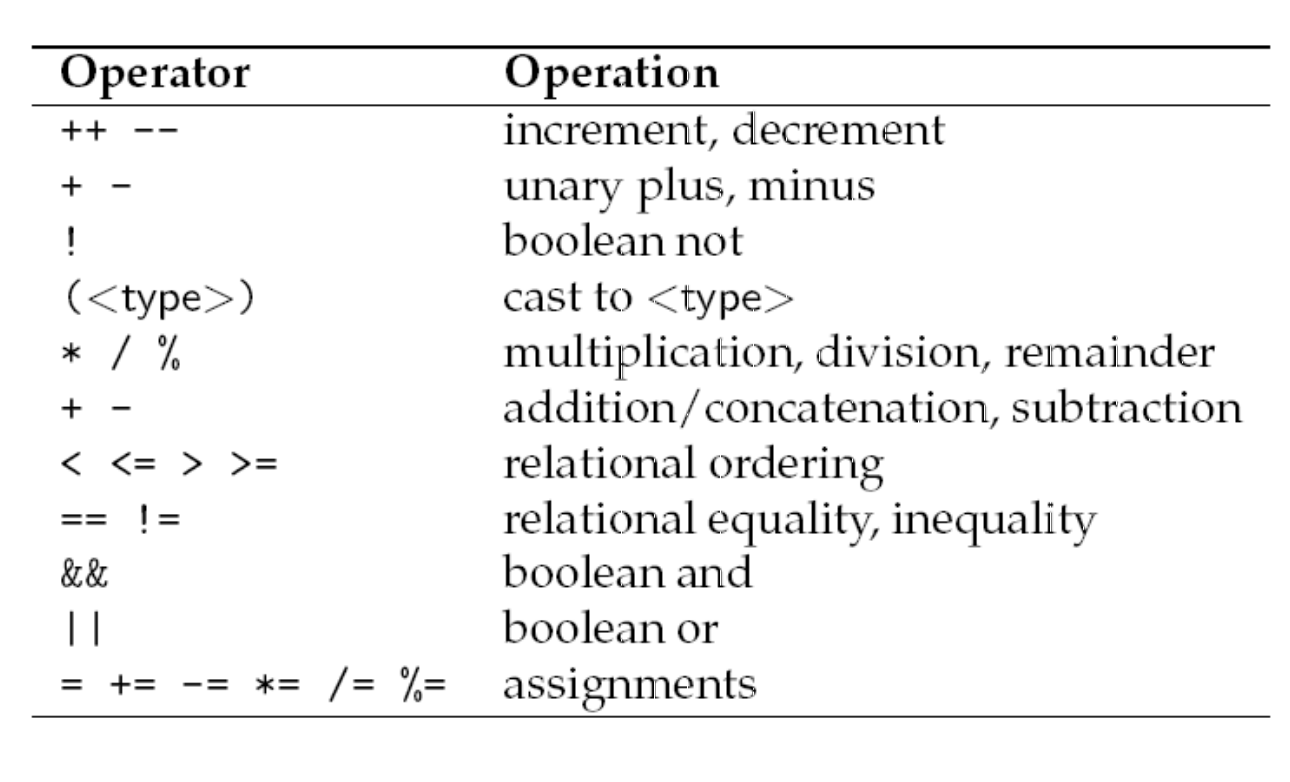
\includegraphics[width=.75\textwidth]{img/c-precedence.png}
  \end{figure}
\end{frame}

\begin{frame}[fragile]
  \frametitle{Relations, No type effect}
  \begin{itemize}
    \item Usual arithmetic conversions are performed on both operands following the
      rules for arithmetic operators.
    \item The values are compared \textbf{\color{Orange} after conversions}.
  \end{itemize}
  \begin{minted}[bgcolor=Black]{c}
int a = 10, b = 20;
float f = 54.677f;
double d = 547.775;
char c1 = 'A', c2 = 'a';
bool b1;

b1 = a == f; // false
b1 = a <= d + 5; // true
b1 = d < c1 * 10; // true
b1 = c1 == c2; // false
b1 = '1' < '2'; // true
b1 = c1 + f < d + a; // true
  \end{minted}
\end{frame}

\begin{frame}[fragile]
  \frametitle{Casting}
  \begin{itemize}
    \item In logical operations
    \begin{itemize}
      \item 0: False
      \item non-zero: True
    \end{itemize}
    \item In mathematical \& comparison operations
    \begin{itemize}
      \item False: 0
      \item True: 1
    \end{itemize}
  \end{itemize}
  \begin{minted}[bgcolor=Black]{c}
bool b1, b2;
int i = 0, j = 20;
b1 = i && j; // b1 = false
b2 = j || j; // b2 = true
i = b1 + b2; // i = 1
j = (i < j) + (b1 && b2); // j = 1
  \end{minted}
\end{frame}

\begin{frame}[fragile]
  \frametitle{Examples}
  \begin{itemize}
    \item x in [10, 20]
    \item \textbf{\color{RubineRed} Wrong Version}
    \begin{itemize}
      \item \mint{c}|10 <= x <= 20|
      \item mint{c}|x = 30|
      \begin{enumerate}
        \item \mint{c}|10 <= 30 <= 20|
        \item \mint{c}|(10 <= 30) <= 20|
        \item \mint{c}|true <= 20|
        \item \mint{c}|1 <= 20|
        \item \mint{c}|true|
      \end{enumerate}
    \end{itemize}
  \end{itemize}
\end{frame}

\begin{frame}[fragile]
  \frametitle{Examples}
  \begin{itemize}
    \item x in [10, 20]
    \item \textbf{\color{LimeGreen} Correct Version}
    \begin{itemize}
      \item \mint{c}|(10 <= x) && (x <= 20)|
      \item \mint{c}|x = 30|
      \begin{enumerate}
        \item \mint{c}|(10 <= 30) && (30 <= 20)|
        \item \mint{c}|true && false|
        \item \mint{c}|false|
      \end{enumerate}
    \end{itemize}
  \end{itemize}
\end{frame}

\begin{frame}[fragile]
  \frametitle{Examples}
  \begin{itemize}
    \item a, b > 0
    \item \textbf{\color{RubineRed} Wrong Version}
    \begin{itemize}
      \item \mint{c}|a && b > 0|
      \item \mint{c}|a = -10; b = 20|
      \begin{enumerate}
        \item \mint{c}|-10 && 20 > 0|
        \item \mint{c}|-10 && (20 > 0)|
        \item \mint{c}|-10 && true|
        \item \mint{c}|true && true|
        \item \mint{c}|true|
      \end{enumerate}
    \end{itemize}
  \end{itemize}
\end{frame}

\begin{frame}[fragile]
  \frametitle{Examples}
  \begin{itemize}
    \item a, b > 0
    \item \textbf{\color{LimeGreen} Correct Version}
    \begin{itemize}
      \item \mint{c}|(a > 0) && (b > 0)|
      \item \mint{c}|a = -10; b = 20|
      \begin{enumerate}
        \item \mint{c}|(-10 > 0) && (20 > 0)|
        \item \mint{c}|false && true|
        \item \mint{c}|false|
      \end{enumerate}
    \end{itemize}
  \end{itemize}
\end{frame}

\section{if-else statement}

\begin{frame}[fragile]
  \frametitle{Type of statements}
  \begin{itemize}
    \item Expression statement
    \begin{itemize}
      \item Single statements
    \end{itemize}
    \begin{minted}[bgcolor=Black]{c}
x = y + 10;
scanf("%d", &i);
    \end{minted}
    \item Control statement
    \begin{itemize}
      \item Control the flow of program
      \item Decisions and loops
    \end{itemize}
    \item Compound statement
    \begin{itemize}
      \item Starts with \{ and ends with \}
      \item All statements can be between \{ and \}
    \end{itemize}
  \end{itemize}
\end{frame}

\begin{frame}[fragile]
  \frametitle{if statement}
  \begin{itemize}
    \item Decision making in C
    \begin{minted}[bgcolor=Black]{c}
if( <expression> )
  <statements1>
else
  <statements2>;
    \end{minted}
    \item Expression
    \begin{itemize}
      \item A boolean statement: \mint{c}|a <= b|
      \item
        A mathematical statement: \mint{c}|a + b| or a variable: \mint{c}|a|
      \begin{itemize}
        \item zero means false
        \item non-zero means true
      \end{itemize}
    \end{itemize}
  \end{itemize}
\end{frame}

\begin{frame}[fragile]
  \frametitle{Even-Odd}
  \begin{minted}[bgcolor=Black]{c}
#include <stdio.h>
int main(void){
  int number_to_test, remainder;
  printf("Enter your number to be tested: ");
  scanf("%d", &number_to_test);
  remainder = number_to_test % 2;
  if(remainder == 0)
    printf ("The number is even.\n");
  else
    printf ("The number is odd.\n");
  return 0;
}
  \end{minted}
\end{frame}

\begin{frame}[fragile]
  \frametitle{Statements in if-else}
  \begin{itemize}
    \item Empty statement
    \begin{minted}[bgcolor=Black]{c}
if(a < b)
  printf("A is larger than b\n");
else
  ;
    \end{minted}
    \item Block statements
    \begin{minted}[bgcolor=Black]{c}
if(a <= b){
  printf("A is less than b or ");
  printf("A is equal b\n");
}
else
  printf("A is greater than b\n");
    \end{minted}
  \end{itemize}
\end{frame}

\begin{frame}[fragile]
  \frametitle{Statements in if-else}
  \scriptsize
  \begin{minted}[bgcolor=Black]{c}
#include <stdio.h>

int main(void){
  int i;
  char c;

  printf("Enter a char: ");
  scanf(" %c", &c);

  printf("Enter an int: ");
  scanf("%d", &i);

  if(i > 0)
    printf("Your number is larger than 0\n");
  else
    printf("Your number is less than or equal 0\n");

  if((c >= '0') && (c <= '9'))
    printf("Your char is Numeric \n");

  return 0;
}
  \end{minted}
\end{frame}

\begin{frame}
  \frametitle{More than two choices}
  \begin{itemize}
    \item If statement: 2 choices
    \begin{itemize}
      \item If conditions are true will run if statements
      \item If conditions are false will run else statements
    \end{itemize}
    \item How to make decisions when there are multiple choices?
  \end{itemize}
\end{frame}

\begin{frame}[fragile]
  \frametitle{Map numeric grade to alphabetic}
  \begin{minted}[bgcolor=Black]{c}
int numg;
char alphag;
if(numg < 25)
  alphag = 'D';
if((numg >= 25) && (numg < 50))
  alphag = 'C';
if((numg >= 50) && (numg < 75))
  alphag = 'B';
if(numg >= 75)
  alphag = 'A';
  \end{minted}
\end{frame}

\begin{frame}
  \frametitle{More than two choices}
  \begin{itemize}
    \item To avoid repeating conditions in if statements
    \item To avoid running unnecessary statements
    \item <span class="hl-red">Nested</span> if: check multiple conditions
    \begin{itemize}
      \item <Statements 1> becomes an if-else statement
      \item <Statements 2> becomes an if-else statement
      \item Repeat it as many as needed
    \end{itemize}
  \end{itemize}
\end{frame}

\begin{frame}[fragile]
  \frametitle{Nested if-else}
  \begin{minted}[bgcolor=Black]{c}
if(c1 && c2)
  s1
if(c1 && !(c2))
  s2
if(!(c1) && c3)
  s3
if(!(c1) && !(c3))
  s4
  \end{minted}
  \begin{minted}[bgcolor=Black]{c}
if(c1)
  if(c2)
    s1
  else
    s2
else
  if(c3)
    s3
  else
    s4
  \end{minted}
\end{frame}

\begin{frame}[fragile]
  \frametitle{Map numeric grade to alphabetic}
  \begin{minted}[bgcolor=Black]{c}
int numg;
char alphag;

if (numg < 25)
  alphag = ‘D’;
else {
  if (numg < 50)
    alphag = ‘C’;
  else {
    if (numg < 75)
      alphag = ‘B’;
    else
      alphag = ‘A’;
  }
}
  \end{minted}
\end{frame}

\begin{frame}[fragile]
  \frametitle{Nested if-else}
  \begin{minted}[bgcolor=Black]{c}
if (<condition 1>)
  <statement 1>
else {
  if(<condition 2>)
    <statement 2>
  else
    <statement 3>
}
  \end{minted}
  \begin{minted}[bgcolor=Black]{c}
if (<condition 1>)
  <statement 1>
else if (<condition 2>)
  <statement 2>
else
  <statement 3>
  \end{minted}
\end{frame}

\begin{frame}[fragile]
  \frametitle{Map numeric grade to alphabetic}
  \begin{minted}[bgcolor=Black]{c}
int numg;
char alphag;

if(numg < 25)
  alphag = 'D';
else if(numg < 50)
  alphag = 'C';
else if(numg < 75)
  alphag = 'B';
else
  alphag = 'A';
  \end{minted}
\end{frame}

\begin{frame}[fragile]
  \frametitle{Nested if: Incomplete branch}
  \begin{enumerate}
    \item \textit{\color{Orange} else} part is optional
    \item
      \textit{\color{Orange} else} always associates with the
      \textit{\color{LimeGreen} nearest}
      \textit{\color{Orange} if}

    \item 1 + 2 can be dangerous specially in incomplete branchs
  \end{enumerate}
  Example: Tell user to move or game over
  \begin{minted}[bgcolor=Black]{c}
if(gameIsOver == 0)
  if(playerToMove == YOU)
    printf ("Your Move\n");
else
  printf ("The game is over\n");
  \end{minted}
  \begin{itemize}
    \item To avoid error you should
    \item Close off you code or Use Empty statements
  \end{itemize}
\end{frame}

\section{switch-case statement}

\begin{frame}[fragile]
  \frametitle{switch-case: Multiple choices}
  \begin{itemize}
    \item Multiple conditions
    \begin{itemize}
      \item if-else if-else if-\ldots
    \end{itemize}
    \item
      Select from alternative \textit{\color{Orange} values} of a
      \textit{\color{LimeGreen} variable}

    \begin{itemize}
      \item switch-case
      \item
        Values should be \textit{\color{Orange} constant} not expression:
        i, i+j,

      \item
        Values \& Variables should be \textit{\color{Orange} int} or
        \textit{\color{Orange} char}

    \end{itemize}
  \end{itemize}
  \begin{minted}[bgcolor=Black]{c}
switch (variable) {
  case value1:
    <statements 1>
  case value2:
    <statements 2>
}
  \end{minted}
\end{frame}

\begin{frame}[fragile]
  \frametitle{How does switch-case work?}
  \begin{itemize}
    \item Each switch-case can be rewritten by if-else
  \end{itemize}
  \begin{minted}[bgcolor=Black]{c}
if(variable == value1){
  <statements 1>
  <statements 2>
}
else if(variable == value2){
  <statements 2>
}
  \end{minted}
\end{frame}

\begin{frame}[fragile]
  \frametitle{switch-case: complete version}
  \scriptsize
  \begin{minted}[bgcolor=Black]{c}
switch(variable) {
  case value1:
    <statements 1>
    break;
  case value2:
    <statements 2>
    break;
  default:
    <statements 3>
}
  \end{minted}
  \scriptsize
  \begin{minted}[bgcolor=Black]{c}
if(variable == value1) {
  <statements 1>
}
else if(variable == value2) {
  <statements 2>
}
else {
  <statements 3>
}
  \end{minted}
\end{frame}

\begin{frame}[fragile]
  \frametitle{switch-case (cont’d)}
  \begin{itemize}
    \item All values used in case should be different
  \end{itemize}
  \begin{minted}[bgcolor=Black]{c}
switch(i){ //Error
case 1:
...
case 2:
...
case 1:
  \end{minted}
\end{frame}

\begin{frame}[fragile]
  \frametitle{switch-case (cont’d)}
  \begin{itemize}
    \item All values must be value, not expression of variables
  \end{itemize}
  \begin{minted}[bgcolor=Black]{c}
switch(i){ //Error
case j:
...
case 2:
...
case k+10:
  \end{minted}
\end{frame}

\begin{frame}[fragile]
  \frametitle{switch-case: multiple matches}
  \scriptsize
  \begin{minted}[bgcolor=Black]{c}
switch(variable) {
  case value1:
  case value2:
    <statements 1>
    break;
  case value3:
    <statements 2>
}
  \end{minted}
  \scriptsize
  \begin{minted}[bgcolor=Black]{c}
if(
  (variable == value1) ||
  (variable == value2)
){
    <statements 1>
} else if (variable == value3) {
    <statements 2>
}
  \end{minted}
\end{frame}

\begin{frame}[fragile]
  \frametitle{switch-case vs. if-else}
  \begin{itemize}
    \item
      \textit{\color{Orange} if-else} is more powerful than
      \textit{\color{Orange} switch-case}

    \item
      \textit{\color{LimeGreen} switch-case} is only for checking the
      \textit{\color{LimeGreen} values of a variable} and the values must be
      \textit{\color{LimeGreen} constant}

    \item if-else is more suitable in some cases, e.g.,
    \begin{minted}[bgcolor=Black]{c}
double var1, var2;
if(var1 <= 1.1)
  <statements 1>
if(var1 == var2)
  <statements 2>
    \end{minted}
  \end{itemize}
\end{frame}

\begin{frame}[fragile]
  \frametitle{Nested switch-case}
  \begin{minted}[bgcolor=Black]{c}
bool b; // b = x && y
switch (x){
  case 0:
    b = 0;
    break;
  case 1:
    switch(y){
      case 0:
        b = 0;
        break;
      case 1:
        b = 1;
        break;
    }
    break;
}
  \end{minted}
\end{frame}

\section{Conditional expressions}

\begin{frame}[fragile]
  \frametitle{Conditional Expression}
  \begin{itemize}
    \item Assign value according to conditions
    \item A ternary operator
  \end{itemize}
  \begin{minted}[bgcolor=Black]{c}
int i, j, k;
bool b;

i = b ? j : k;
  \end{minted}
  \begin{minted}[bgcolor=Black]{c}
if (b)
  i = j;
else
  i = k;
  \end{minted}
\end{frame}

\begin{frame}[fragile]
  \frametitle{Conditional Expression: Examples}
  \begin{minted}[bgcolor=Black]{c}
y = (x > 0) ? x : -x

sign = (x < 0) ? -1 : ((x > 0) ? 1 : 0)
  \end{minted}
\end{frame}

\section{Common Bugs}

\begin{frame}[fragile]
  \frametitle{Common Bugs}
  \begin{itemize}
    \item Equality of floating point numbers
    \item
      Two float numbers may or may \textbf{\color{RubineRed} NOT} be equal
  \end{itemize}
  \begin{minted}[bgcolor=Black]{c}
double d1, d2;
d1 = 1e20 + 1;
d2 = 1e20 - 1;
if(d1 == d2)
  printf("They are equal :-o \n");
else
  printf("They are not equal :D \n");
  \end{minted}
  \begin{block}{}
  They are equal :-o
  \end{block}
\end{frame}

\begin{frame}[fragile]
  \begin{block}{}
    Instead of checking for equality, check their difference to be in a
    small-enough period.
  \end{block}
  \begin{minted}[bgcolor=Black]{c}
double d1, d2;
d1 = 1e20 + 1;
d2 = 1e20 - 1;
if(fabs(d1 - d2) <= 0.0000001)
  printf("They are equal :-o \n");
else
  printf("They are not equal :D \n");
  \end{minted}
\end{frame}

\begin{frame}[fragile]
  \frametitle{Common Bugs}
  \begin{itemize}
    \item Danger of empty statement
    \item Danger of assignment (=) and equality (==)
    \begin{minted}[bgcolor=Black]{c}
int a = 10;
int b = 20;
if (a = b) // logical but not compile error!!!
    \end{minted}
    \item Danger of similarity between C and mathematic
    \begin{minted}[bgcolor=Black]{c}
if (a < b < c) // Logical Error
if (a && b < 0) // Logical Error
    \end{minted}
  \end{itemize}
\end{frame}

\begin{frame}
  \frametitle{Avoiding Bugs}
  \begin{itemize}
    \item Precedence of operators
    \item Use parenthesis in conditions
    \item Close-off code as much as you can
  \end{itemize}
\end{frame}

\begin{frame}
  \frametitle{Debugging by assert}
  \begin{itemize}
    \item
      The assert macro is defined in \textit{\color{Orange} assert.h}
    \item assert(an expression)
    \begin{itemize}
      \item If the expression is true: nothing
      \item If the expression is false: error message + halt
    \end{itemize}
  \end{itemize}
\end{frame}

\begin{frame}
  \frametitle{Legends}
  \begin{figure}
    
\includegraphics[height=.75\textheight]{./img/coronavirus.jpg}
  \end{figure}
  \pause%
  \centering
  \color{Violet} COVID-19
\end{frame}


\end{document}
